% !TEX TS-program = pdflatex
% !TEX encoding = UTF-8 Unicode

\documentclass[handout,svgnames]{beamer}
%\documentclass{beamer}

%\usepackage{pgfpages} %for {show notes on second screen option}

\mode<presentation>
{
  %\usetheme{Rochester} %pretty plain, no footer and progress
  %\usetheme{Marburg}   %sidebar with all (sub)sections
  %\usetheme{Madrid}	%footer with author, title, date and frame number, 
  %\usetheme{Luebeck}		%big header with all sections, footer with author and title
  \usetheme{Frankfurt}  %favorite for now %header with progress
  %\usetheme{Dresden}	%header with progress, 2 footers for author an title
  %\usetheme{Copenhagen}	%big header with all sections, footer with author and title
  %\usetheme{Berlin}		%header with progress, 2 footers for author an title
  %\usetheme{Warsaw}		%big header with all sections, footer with author and title
%\setbeamercolor*{palette primary}{use=structure,fg=white,bg=DarkGreen}
\useinnertheme{circles} %bullet points look nice to me that way (especially numbered ones)

  %\setbeamercovered{transparent}
  % or whatever (possibly just delete it)

\setbeamertemplate{navigation symbols}{}%remove navigation symbols
%\setbeameroption{show notes on second screen}
}

\usepackage[ngerman]{babel}
\usepackage[utf8x]{inputenc}
\usepackage[T1]{fontenc}
\usepackage{eurosym} %for euro symbol via \euro

\usepackage{graphicx}
\usepackage{wrapfig}


%code listing stuff
\usepackage{listings}
%\usepackage{color}
\definecolor{mygreen}{rgb}{0,0.6,0}
\definecolor{mygray}{rgb}{0.5,0.5,0.5}
\definecolor{mymauve}{rgb}{0.58,0,0.82}
\lstset{ %
backgroundcolor=\color{white},   % choose the background color; you must add \usepackage{color} or \usepackage{xcolor}
basicstyle=\footnotesize,        % the size of the fonts that are used for the code
breakatwhitespace=false,         % sets if automatic breaks should only happen at whitespace
breaklines=true,                 % sets automatic line breaking
%  captionpos=b,                    % sets the caption-position to bottom
commentstyle=\color{mygreen},    % comment style
deletekeywords={...},            % if you want to delete keywords from the given language
escapeinside={\%*}{*)},          % if you want to add LaTeX within your code
extendedchars=true,              % lets you use non-ASCII characters; for 8-bits encodings only, does not work with UTF-8
frame=single,                    % adds a frame around the code
keepspaces=true,                 % keeps spaces in text, useful for keeping indentation of code (possibly needs columns=flexible)
keywordstyle=\color{mygreen},       % keyword style
language=Cobol,                 % the language of the code
morekeywords={*,...},            % if you want to add more keywords to the set
numbers=none,                    % where to put the line-numbers; possible values are (none, left, right)
numbersep=5pt,                   % how far the line-numbers are from the code
numberstyle=\tiny\color{mygray}, % the style that is used for the line-numbers
rulecolor=\color{black},         % if not set, the frame-color may be changed on line-breaks within not-black text (e.g. comments (green here))
showspaces=false,                % show spaces everywhere adding particular underscores; it overrides 'showstringspaces'
showstringspaces=false,          % underline spaces within strings only
showtabs=false,                  % show tabs within strings adding particular underscores
stepnumber=2,                    % the step between two line-numbers. If it's 1, each line will be numbered
stringstyle=\ttfamily\color{red},     % string literal style
tabsize=2,                       % sets default tabsize to 2 spaces
title=\lstname                   % show the filename of files included with \lstinputlisting; also try caption instead of title
}

%stuff used for the tables
\usepackage{tabularx}
\usepackage{hhline}
\newcommand{\mcc}[2]{\multicolumn{#1}{|c|}{#2}} %multirows over X rows in tabularx

\newcommand{\hilight}[1]{\colorbox{yellow}{#1}} %command for magic marker highlighting
%   (from http://pleasemakeanote.blogspot.de/2009/08/how-to-highlight-text-in-latex.html)

\title[OpenLDAP- und FreeRADIUS-Server]   % (optional, use only with long paper titles)
{LDAP+RADIUS}

\subtitle
{Identity Management für Masochisten} % (optional)

\author % (optional, use only with lots of authors)
{Sebastian Deußer}
%\date{13. Juli 2015}


%\subject{COBOL \"Ubersicht}
% This is only inserted into the PDF information catalog. Can be left
% out. 

% If you have a file called "university-logo-filename.xxx", where xxx
% is a graphic format that can be processed by latex or pdflatex,
% resp., then you can add a logo as follows:

% \pgfdeclareimage[height=0.5cm]{university-logo}{university-logo-filename}
% \logo{\pgfuseimage{university-logo}}

% If you wish to uncover everything in a step-wise fashion, uncomment
% the following command: 
%\beamerdefaultoverlayspecification{<+->}


\begin{document}
\setcounter{framenumber}{-1}
\frame{\titlepage}
\setbeamertemplate{footline}[frame number] %show page numbers in footer
%\begin{frame}[noframenumbering]
%  \titlepage
%\end{frame}

\section{}
\begin{frame}{Übersicht}
\tableofcontents
%	\begin{enumerate}
%		\item Projektbeschreibung
%		\begin{itemize}
%			\item Projektumfeld
%			\item Projektthema
%		\end{itemize}
%		\item Planung
%		\begin{itemize}
%			\item Planung Ersatzserver
%			\item Kommunikationskonzept
%		\end{itemize}
%		\item Realisierung
%		\begin{itemize}
%			\item OpenLDAP-Server
%			\item FreeRADIUS-Server
%		\end{itemize}
%		\item Projektkosten
%		\item Abschluss
%		\begin{itemize}
%			\item Fazit
%			\item Ausblick
%		\end{itemize}
%	\end{enumerate}
\end{frame}
\note{}

\section{Projektbeschreibung}
\subsection{Ausgangssituation}
\begin{frame}{Projektumfeld: Firmenbeschreibung fgn GmbH}
\begin{figure}[htbp] 
	\centering
	
\includegraphics[scale=0.75]{Bilder/logo_fgn.png}
%	\caption{Logo der fgn GmbH}
	\label{fig:fgn-Logo}
\end{figure}
\begin{itemize}
	\item Praktikumsbetrieb fgn GmbH gegründet 1996 SpinOff der TU Kaiserslautern
	\item Kerngeschäft Netzwerkschulungen und -consulting (herstellerunabhängig)
	\item circa ein Dutzend Mitarbeiter (ungefähr gleich verteilt auf Trainer, Consulting, Verwaltung/Administration)
	\item eigene Schulungslabore (Remote Labs) mit Managed Switches und VMs auf ESXi-Servern
	\item Büro- und Server-Räume in DFKI Neubau, deswegen Internetanbindung über TU Kaiserslautern
%	\item öffentliche Webseite extern gehostet, restliche Server selbst verwaltet in Server-Räumen im DFKI
%	\item meisten Server sind VMs auf ESXi-Servern
%	\item Schulungslabore (Remote Labs) mit eigenen Managed Switches und ESXi-Servern in eigenem VPN, Zugang über OpenVPN (Telnet für Switches, Remote Desktop für Windows VMs)
\end{itemize}
\end{frame}


\begin{frame}{Ausgangssituation}
\begin{itemize}
	\item CommuniGate-Server für E-Mail und Identity Management
	\item Identity Management genutzt von:
	\begin{itemize}
		\item E-Mail
		\item firmeninterne Webtools (z.B. Nagios, Trac)
		\item OpenVPN-Server
		\item Egroupware
	\end{itemize}
	\item CommuniGate stark veraltet, deswegen SSL-Probleme (und vermutlich etliche Sicherheitslücken)
\end{itemize}
\end{frame}


\section{Planung}
%\subsection{Konzeptplanung}
\subsection{}
\begin{frame}{Konzept Ersatzserver}

\end{frame}


\begin{frame}{Kommunikation der Server untereinander}

\end{frame}


\section{Realisierung}
\subsection{Realisierung von LDAP}
\begin{frame}{Realisierung von LDAP}
\end{frame}

\begin{frame}{Endgültiger LDAP-Verzeichnisbaum}
%	\begin{figure}[htbp] 
%		\centering
		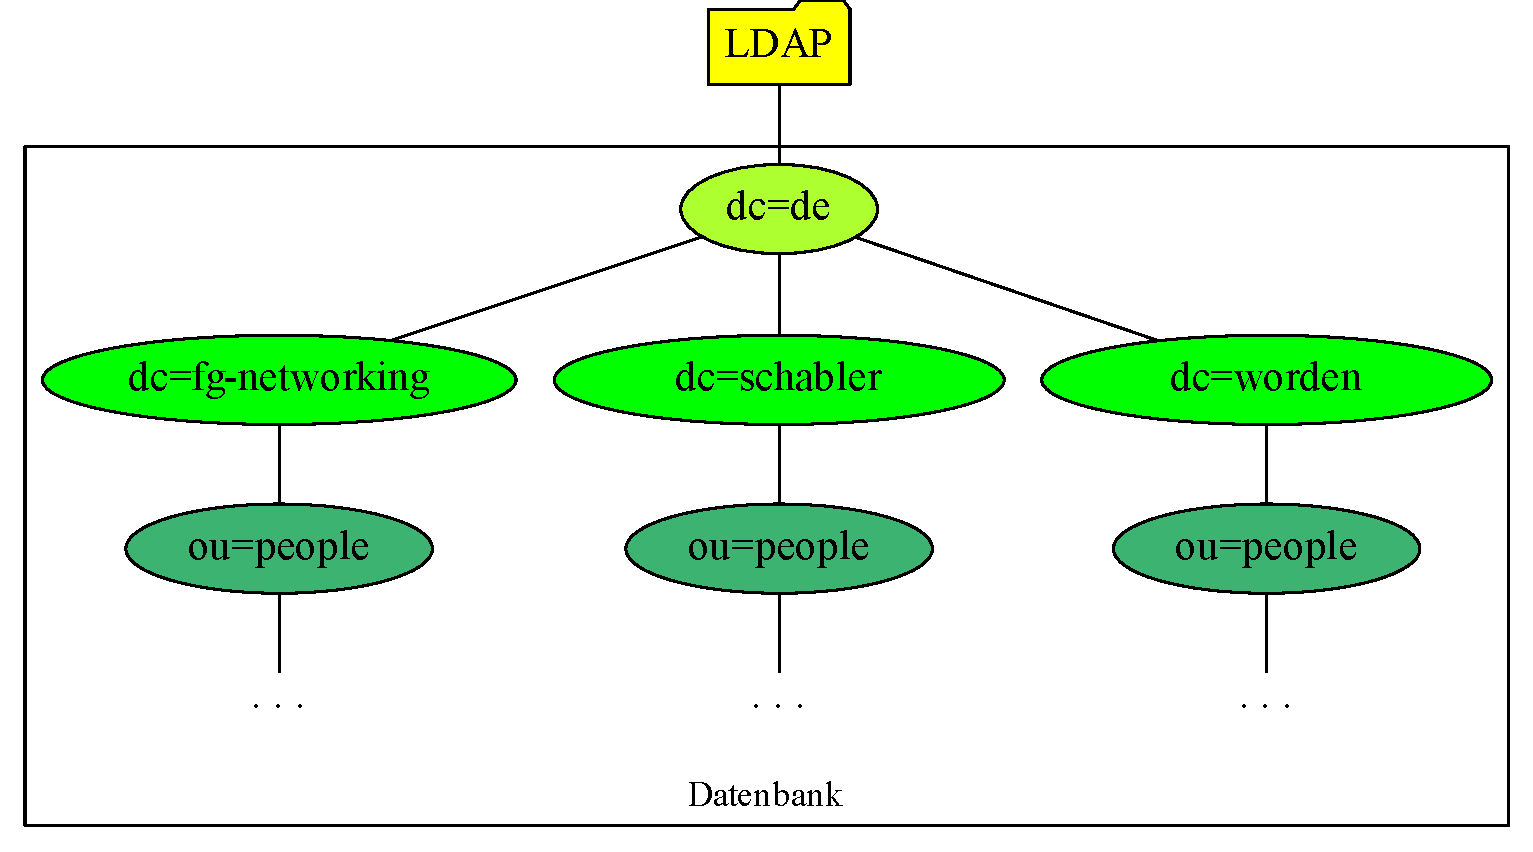
\includegraphics[width=\textwidth]{Bilder/LDAP-fgn.pdf}
%		\caption{Der fertige LDAP-Verzeichnisbaum}
%		\label{fig:LDAP-Baum}
%	\end{figure}
\end{frame}


\subsection{Realisierung von RADIUS}
\begin{frame}{Realisierung von RADIUS}

\end{frame}


\begin{frame}{Qualitätssicherung/-tests}

\end{frame}


\subsection{Probleme und Lösungen}
\begin{frame}{Probleme und Lösungen}

\end{frame}


\section{Projektkosten}
\subsection{Projektkosten - Anschaffung}
\begin{frame}{Projektkosten - Anschaffung}
	\begin{tabularx}{\textwidth}{|X|r|r|r|}
%		\hline
%		\mcc{4}{Kosten für die Einrichtung}\\
		\hline
		Kosten-	&	OpenLDAP \& &	\centering CommuniGate- &	\\
		Kategorie	&	FreeRADIUS &	\centering Upgrade &	Status Quo\\
		\hline
		Hardware &	0,00\euro{} &	0,00\euro{} &	0,00\euro{}\\
		\hline
		Softwarelizenzen &	0,00\euro{} &	1.849,00\euro{} &	0,00\euro{}\\
		\hline
		Arbeitsaufwand &	2.485,00\euro{} &	2.485,00\euro{} &	0,00\euro{}\\
		\hhline{|=|=|=|=|}
		Gesamt &	2.485,00\euro{} &	4.334,00\euro{} &	0,00\euro{}\\
		\hline
	\end{tabularx}
\end{frame}


\subsection{Projektkosten - Wartung}
\begin{frame}{Projektkosten - Wartung}
	\begin{tabularx}{\textwidth}{|X|r|r|r|}
%		\hline
%		\mcc{4}{Jährliche Kosten}\\
		\hline
		Kosten-	&	OpenLDAP \& &	CommuniGate- &	\\
		Kategorie	&	FreeRADIUS &	Upgrade &	Status Quo\\
		\hline
		Hardware &	0,00\euro{} &	0,00\euro{} &	0,00\euro{}\\
		\hline
		Softwarelizenzen &	0,00\euro{} &	332,82\euro{} &	0,00\euro{}\\
		\hline
		Arbeitsaufwand &	355,00\euro{} &	213,00\euro{} &	2.350,00\euro{}\\
		\hhline{|=|=|=|=|}
		Gesamt &	355,00\euro{} &	545,82\euro{} &	2.350,00\euro{}\\
		\hline
	\end{tabularx}
\end{frame}


\section{Projektabschluss}
\subsection{Fazit}
\begin{frame}{Fazit}

\end{frame}


\subsection{Ausblick}
\begin{frame}{Ausblick}
	Erweiterungsmöglichkeiten
	\begin{enumerate}
		\item Anbindung neue E-Mailserver (\texttt{postfix})
		\item Ersatz lokale Accounts
		\item Anbindung Managed Switches über RADIUS
		\item Samba 4 Domäne für Windows Rechner
	\end{enumerate}
\end{frame}

\section{}%section shall not be visible in navbar, hence empty name
\begin{frame}{Quellen}
	Vielen Dank für Ihre Aufmerksamkeit
	
	\medskip Diese Präsentation wurde mit \LaTeX{}-Beamer erstellt
\end{frame}


%\section{Übersicht}
%\subsection{Namensbedeutung}
%\begin{frame}{Namensbedeutung}
%	\begin{columns}[c]%sort the graphics with columns
%		\begin{column}{4cm}
%			
\includegraphics[width=4cm]{CobolCogLogo}\\ 
%			
\includegraphics[width=4cm]{GnuCOBOLLogoTransparent}
%		\end{column}
%		\begin{column}{6cm}
%			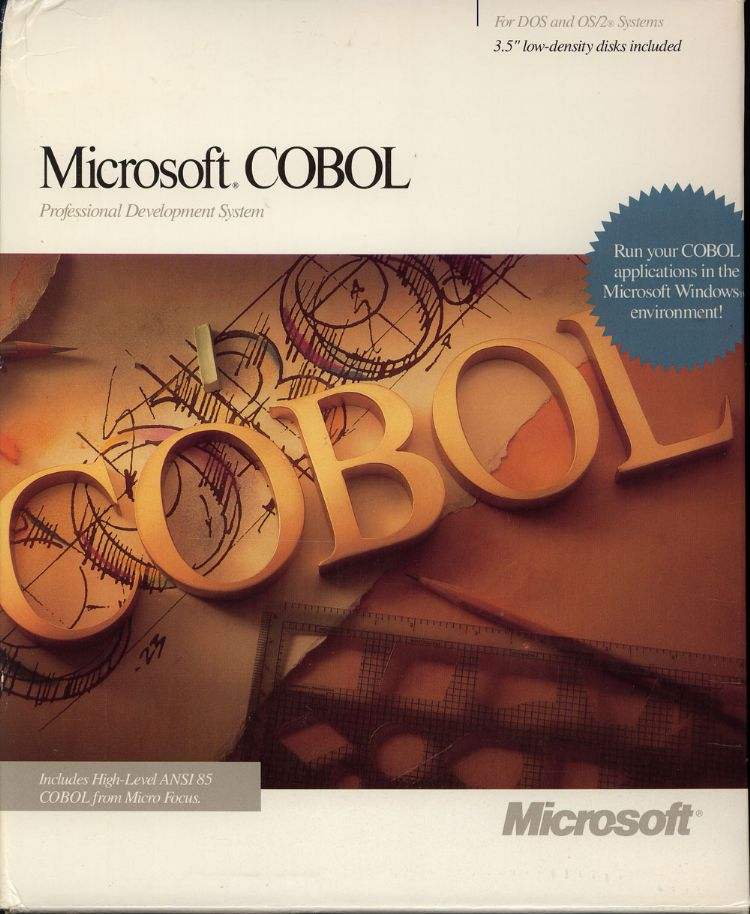
\includegraphics[width=2.5cm]{DOSMSCOBOL45} \hspace{1.5pt}
%			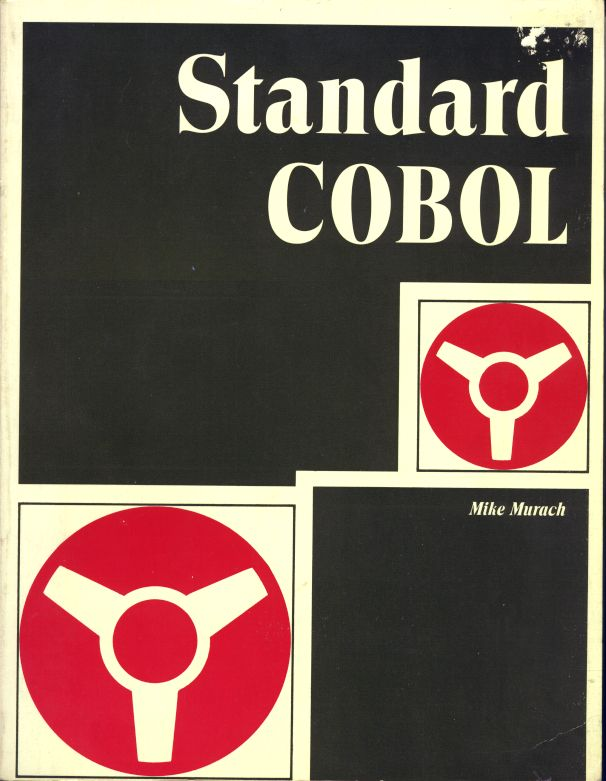
\includegraphics[width=2.5cm]{StandardCobol}
%		\end{column}
%	\end{columns}
%	\pause
%	\begin{itemize}[<+->]%auto-generate pause after each item
%		\item
%			COBOL steht für COmmon Business-Oriented Language.
%		\item
%			entwickelt für betriebswirtschaftliche Programme (im Gegensatz zum technisch-wissenschaftlichen Fokus anderer Sprachen)
%	\end{itemize}
%\end{frame}
%\note{4 Grafiken plus 2}
%
%\subsection{Historische Entwicklung}
%\begin{frame}{Anfänge}
%	\begin{itemize}[<+->]
%		\item
%			entwickelt durch Arbeitsgruppe in der 2. H\"alfte von 1959
%		\item%here comes some tricky stuff to position a picture next to text in an itemize environment
%  \begin{minipage}[t]{0.7\textwidth}
%%	\vspace{-5pt}
%	federführend war Grace Hopper, Erfinderin des ersten Compilers (A-0) und Mitentwicklerin fr\"uher Computer (z.B. Harvard Mark I+II, UNIVAC I)
%	\end{minipage}\hspace{2pt}
%	\begin{minipage}[t]{0.15\textwidth}
%	\vspace{-12pt}%\raggedright
%    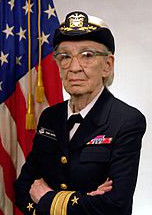
\includegraphics[width=1.5cm]{Grace_Hopper_small}
%	\end{minipage}
%		\item
%			basierte auf Hoppers FLOW-MATIC, IBMs COMTRAN (``Business-Version'' von FORTRAN) und Honeywells FACT
%		\item
%		erster Standard (COBOL 60) festgelegt am 03. Januar 1960, danach individuelle (inkompatible) Erweiterungen von verschiedenen Firmen
%	\end{itemize}
%\end{frame}
%\note{4}
%
%\begin{frame}{Versionen des Standards}
%	\begin{itemize}[<+->]
%		\item
%			ANS COBOL 1968: ANSI Standard um die verschiedenen \"Anderungen nach 1959 zu einer neuen Basis zusammenzufassen
%		\item
%			COBOL 1974: 2. ANSI Standard, neue Features wie Datei-Organisation, Report Modul; Einführung der Möglichkeit ein Programm in Funktionen zu unterteilen; Abschaffung von Features, deshalb inkompatibel zu vorherigen Standards
%		\item
%			COBOL 1985: \"uberarbeiteter ANSI Standard, Einf\"uhrung G\"ultigkeitsbereich-Terminatoren (z.B. \texttt{END-IF}), neue Features geschachtelte Unterprogramme, neue Statements, die Operatoren >= und <=; ersetzen von selbstmodifizierenden Code (\texttt{ALTER}) durch Referenz Modifikation
%	\end{itemize}
%\end{frame}
%\note{4}
%
%\begin{frame}{Entwicklung um und nach 2000}
%	\begin{itemize}[<+->]
%		\item
%			viele Programm aus den 80ern und davor verwendeten in Records Datumsfelder mit fester 2-stelliger Jahreszahl
%		\item
%			=> um 1999/2000 Massensterben unter COBOL Anwendungen wegen Y2K-Bug; Programme mussten entweder grundlegend überarbeitet oder ganz ersetzt werden
%		\item
%			COBOL 2002: neue zeitgemäße Features wie Locale/Unicode-Unterstützung, Objektorientierung zur Einbindung in Java und .NET-Frameworks, Fließkommaunterstützung
%		\item
%			Ausblick: COBOL 20XX Standard in Entwicklung (erwartet 2014-6), baut primär Objektorientierung aus und passt Datentypen an neue Standards an
%		\end{itemize}
%\end{frame}
%\note{4}
%
%\section{Einsatz}
%\subsection{Einsatzgebiete}
%\begin{frame}{Einsatzgebiete}
%	\pause
%	\begin{columns}[t]
%		\begin{column}{4cm}
%			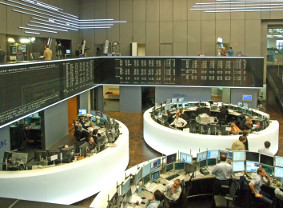
\includegraphics[width=4cm]{Deutsche-boerse}
%		\end{column}
%	\pause
%		\begin{column}{3cm}
%			
\includegraphics[width=3cm]{sparda_logo}
%		\end{column}
%	\pause
%		\begin{column}{3.5cm}
%			
\includegraphics[width=3.5cm]{california-state-flag1} 
%		\end{column}
%	\end{columns}
%	\pause
%	\begin{itemize}[<+->]
%		\item
%			Haupteinsatzgebiet ist betriebswirtschaftliche Datenverarbeitung (z.B. Gehaltsabrechnungen, Touristik)
%		\item
%			bei klassischer Aufteilung nach Benutzerschnittstelle, Verabreitungsteil und Datenhaltungsteil stellt COBOL den Verarbeitungsteil eines EDV-Programms
%	\end{itemize}
%\end{frame}
%\note{3 Grafiken plus 2}
%
%\subsection{heutiger Einsatz}
%\begin{frame}{heutiger Einsatz}
%	\begin{itemize}[<+->]
%		\item
%			COBOL hatte wenig Einfluss auf sp\"atere Programmiersprachen da Fokus auf relativ simple Algorithmen und hohes I/O-Volumen akademisch uninteressant (Ausnahme: SAPs Programmiersprache ABAP)
%		\item
%			geschätzte 70-80\% aller Geschäftstransaktion involvieren COBOL Programme, oft als Teil von jahrzehntelang gewachsenen Systemen
%		\item
%			komplette Neuentwicklungen nur noch selten in COBOL
%		\item
%			2010 geschätzt \"uber 40 Milliarden Zeilen COBOL Code in Industrieprogrammen verwendet, Wachstumsrate 4 Milliarden Zeilen Code pro Jahr
%	\end{itemize}
%\end{frame}
%\note{4
%		\begin{itemize}
%			\item
%			
%			\item
%				täglich 200 mal mehr COBOL-Transaktion als Google Suchanfragen
%			\item
%				primär Erweiterungen alter Systeme
%			\item
%				1997 schätze Gartner noch 200 Mrd Zeilen bei 5 Mrd Wachstum
%		\end{itemize}}
%
%\section{Vor- und Nachteile}
%\subsection{Vorteile}
%\begin{frame}{Vorteile}
%	\begin{itemize}[<+->]
%		\item
%			entworfen um Programme auf verschiedener Hardware laufen zu lassen ohne große Ver\"anderung des Codes
%		\item
%			durch mehrstufiges Design der einzelnen Programmsprachen-Module lassen sich COBOL-Programme auf sehr eingeschr\"ankter Hardware mit geringen Anpassungen ausf\"uhren
%		\item
%			der ANSI-Standard wird durchschnittlich alle 10-15 Jahre an neue Gegebenheiten angepasst, z.B. kam 2002 Unterstüzung für Objektorientierung dazu
%		\item
%			es gibt einen kostenlosen quelloffenen Compiler namens GNU COBOL (ehemals OpenCOBOL) für POSIX-kompatible Betriebssysteme
%	\end{itemize}
%\end{frame}
%\note{4}
%
%\subsection{Nachteile}
%\begin{frame}{Nachteile}
%	\begin{itemize}[<+->]
%		\item
%		    bis COBOL 74 gab es keine M\"oglichkeit Programme zu strukturieren, z.B. waren alle Variablen global
%		\item
%			aufgrund vieler Eigenentwicklungen von Firmen und anderen Gruppen gibt es viele verschiedene Standards von COBOL die teilweise inkompatibel zueinander sind
%		\item
%			da die Syntax sich an geschriebenem Englisch orientiert werden COBOL Programme schnell recht langwierig zu schreiben
%		\item
%			COBOL Programmierer sterben langsam aus
%	\end{itemize}
%\end{frame}
%\note{4}
%
%\section{Praxis}
%\subsection{Entwicklungsumgebung}
%\begin{frame}{Entwicklungsumgebung}
%	\begin{itemize}[<+->]
%		\item
%			viele Computer/Betriebsystemhersteller (z.B. IBM, Siemens, Unisys, HP) entwickelten (und vertreiben teilweise immer noch) eigene Compiler, oft mit eigenen Erweiterungen des Standards
%		\item
%			es gibt verschiedene Codegeneratoren die COBOL-Programme oder Teile davon generieren um die Entwicklungsarbeit zu erleichtern
%		\item
%			Plugins für viele gängige IDEs, z.B. cobolclipse für Eclipse
%	\end{itemize}
%\end{frame}
%\note{3}
%
%\begin{frame}{Entwicklungsumgebung (2)}
%	\begin{itemize}
%		\item
%			verbreiteste (kommerzielle) COBOL IDE ist Visual COBOL von Micro Focus; besitzt moderne Features wie Generierung von Java Byte-Code, .NET Unterstützung und Webservices
%		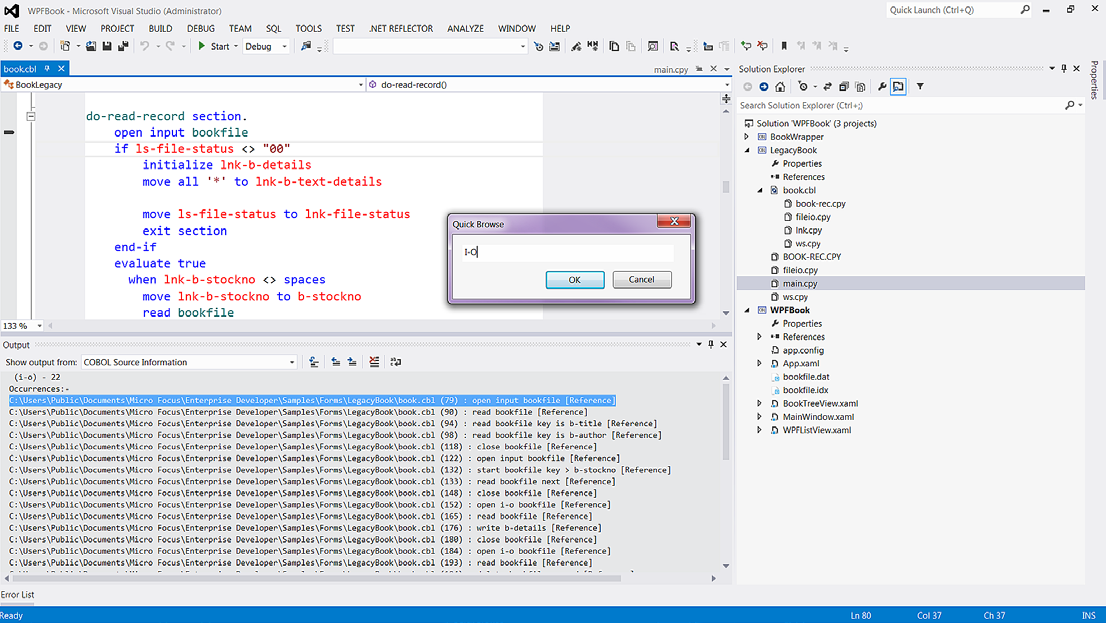
\includegraphics[width=9cm]{VisualCOBOL2}
%	\end{itemize}
%\end{frame}
%
%
%\subsection{Sprachspezifikation}
%\begin{frame}{Sprachspezifikation}
%	\begin{itemize}[<+->]
%		\item
%			COBOL wurde so entworfen das der Code relativ lesbarem Englisch entspricht z.B. ``\texttt{ADD b TO c GIVING a}'' (a = b + c)
%		\item
%			importieren von Programmteilen als sgn. Copybooks mit \texttt{COPY} Befehl, vergleichbar mit \texttt{\#include} in C u.\"A.
%		\item
%			Kontrollstrukturen:
%			\begin{itemize}[<+->]
%				\item \texttt{IF...ELSE}: funktioniert wie erwartet
%				\item \texttt{EVALUATE}: vergleichbar mit CASE/Switch (eingeführt mit COBOL 85)
%				\item \texttt{PERFORM}: vergleichbar mit for-Schleifen
%				\item \texttt{GO TO}: Standard GOTO, optional mit Bedingung
%			\end{itemize}
%	\end{itemize}
%\end{frame}
%\note{3+4}
%
%\begin{frame}{Datenstrukturen}
%	\begin{itemize}[<+->]
%		\item
%			Grunddatenstruktur ist ein sogenannter Record, ein multidimensionales heterogenes Array
%		\item
%			Records k\"onnen mit homogenen Arrays gemischt verwendet werden, ein Array kann also Inhalt eines Records sein und umgekehrt
%		\item
%			über die \texttt{PICTURE} Klausel kann man den Inhalt (inklusive Feldgrößen) von Records exakt definieren
%		\item
%			Variablen müssen bei der Deklaration typisiert werden, allerdings hat man Dank Records und der \texttt{PICTURE} Klausel vergleichsweise viel Freiheit dabei
%	\end{itemize}
%\end{frame}
%\note{4}
%
%\begin{frame}{Aufteilung eines Programms}
%	\begin{itemize}[<+->]
%		\item
%			jedes Programm besteht aus 4 Teilen (\texttt{DIVISION}) zur Trennung von:
%			\begin{itemize}[<+->]
%			 	\item hardwareabh\"angigem und unabh\"angigem Code
%				\item Algorithmen Beschreibungen und Daten Beschreibungen
%			 \end{itemize}
%		\item
%			\texttt{IDENTIFICATION}: beginnt jedes Programm, benennt Programm und den Autor (Autor optional), sonstige Kommentare als Dokumentation
%		\item
%			\texttt{ENVIRONMENT}: beinhaltet maschinenabhängige Programmspezifikationen wie z.B. Verbindungen zwischen dem Programm und externen Daten
%		\item
%			\texttt{PROCEDURE}: beinhaltet die Algorithmen
%		\item
%			\texttt{DATA}: beinhaltet die Daten Beschreibungen
%	\end{itemize}
%\end{frame}
%\note{1+2,4}
%
%\setbeamercovered{transparent}
%\def\beamertemplatetransparentcoveredmedium{\setbeamercovered{transparent=20}}
%\beamertemplatetransparentcoveredmedium %covered stuff is now only semi-transparent
%\begin{frame}[fragile]{Code-Beispiele}
%	\onslide<1-1>%Listing 1 only fully visible on slide 1
%	\noindent\begin{minipage}{.44\textwidth}
%		\begin{lstlisting}{Hello World}
%			IDENTIFICATION DIVISION.
%			PROGRAM-ID. HELLO-WORLD.
%			PROCEDURE DIVISION.
%			 DISPLAY "Hello, world."
%			 STOP RUN.
%		\end{lstlisting}
%	\end{minipage}\hfill\pause
%	\onslide<2-2>
%	\noindent\begin{minipage}{.53\textwidth}
%		\begin{lstlisting}{Schleifen}
%			PERFORM VARYING i FROM 0 BY 1
%			 UNTIL i >= 10
%			 DISPLAY i
%			END-PERFORM
%		\end{lstlisting}
%	\end{minipage}\pause
%	\onslide<3-3>
%	\lstset{numbers=left,firstnumber=1}
%	\begin{lstlisting}{EVALUATE}
%		EVALUATE True
%		 WHEN Nenner > 0
%		  COMPUTE Zahl = Zaehler / Nenner
%		 WHEN Nenner < 0
%		  COMPUTE Zahl = Zaehler / Nenner * -1
%		 WHEN OTHER
%		  DISPLAY "Fehler"
%		  MOVE 0 TO Zaehler
%		END-EVALUATE
%	\end{lstlisting}
%\end{frame}
%\note{3 Listings}
%
%\section{}%section shall not be visible in navbar, hence empty name
%\begin{frame}{Quellen}
%	\begin{enumerate}
%		\item COBOL Artikel englische Wikipedia
%			\url{http://en.wikipedia.org/wiki/COBOL}
%		\item COBOL Artikel deutsche Wikipedia
%			\url{http://de.wikipedia.org/wiki/COBOL}
%		\item
%			Terrence W. Pratt - Programming Languages: Design and Implementation (Prentice Hill 1975)
%		\item OpenCOBOL Programmers Guide \url{http://opencobol.add1tocobol.com/OpenCOBOL\%20Programmers\%20Guide.pdf}
%	\end{enumerate}
%\end{frame}

\end{document}
